\documentclass{standalone}
\usepackage{pgfplots}

\begin{document}
	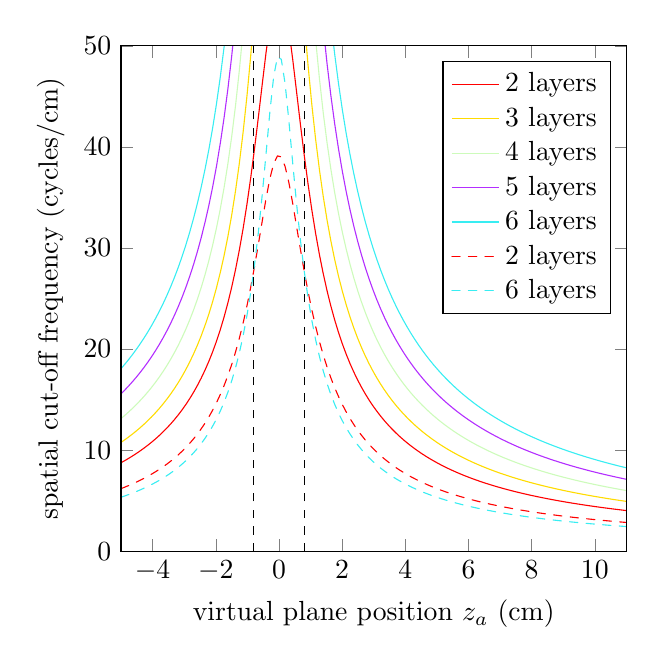
\begin{tikzpicture}
	
		\definecolor{c1}{RGB}{255, 0, 0}
		\definecolor{c2}{RGB}{255, 219, 0}
		\definecolor{c3}{RGB}{205, 251, 187}
		\definecolor{c4}{RGB}{56, 237, 242}
		\definecolor{c5}{RGB}{179, 46, 255}
	
		\pgfplotscreateplotcyclelist{mycolors}{c1, c2, c3, c5, c4, c5, c4}
		
		\begin{axis}[	legend pos = north east, 
						ymin = 0,
						ymax = 50, 
						xmin = -5,
						xmax = 11,
						domain = -5 : 13,
						xtick = {-4, -2, 0, 2, 4, 6, 8, 10, 12},
						ylabel = {spatial cut-off frequency (cycles/cm)},
						xlabel = {virtual plane position $z_a$ (cm)},
						ylabel near ticks,
						no markers,
						samples = 150, 
						cycle list name = mycolors,
						axis on top = true,
						width = 8 cm, 
						height = 8 cm]
		
			% f_0 = 27.7 cycles/cm
			% h = 1.6 cm
		
			\addplot{2 * 27.7 * sqrt( (2 + 1) * 1.6^2 / ( (2 + 1) * 1.6^2 + 12 * (2 - 1) * (x^2) ) )};
			\addlegendentry{2 layers};
			
			\addplot{3 * 27.7 * sqrt( (3 + 1) * 1.6^2 / ( (3 + 1) * 1.6^2 + 12 * (3 - 1) * (x^2) ) )};
			\addlegendentry{3 layers};
			
			\addplot{4 * 27.7 * sqrt( (4 + 1) * 1.6^2 / ( (4 + 1) * 1.6^2 + 12 * (4 - 1) * (x^2) ) )};
			\addlegendentry{4 layers};
			
			\addplot{5 * 27.7 * sqrt( (5 + 1) * 1.6^2 / ( (5 + 1) * 1.6^2 + 12 * (5 - 1) * (x^2) ) )};
			\addlegendentry{5 layers};
			
			\addplot{6 * 27.7 * sqrt( (6 + 1) * 1.6^2 / ( (6 + 1) * 1.6^2 + 12 * (6 - 1) * (x^2) ) )};
			\addlegendentry{6 layers};
			
			\addplot[dashed, cap = round, c1]{27.7 * sqrt( 2 * (2 * 2 - 1) * 1.6^2 / ( (2 + 1) * 1.6^2 + 12 * (2 - 1) * (x^2) ) )};
			\addlegendentry{2 layers};
			
%			\addplot[dotted, cap = round, c2]{27.7 * sqrt( 2 * (2 * 3 - 1) * 1.6^2 / ( (3 + 1) * 1.6^2 + 12 * (3 - 1) * (x^2) ) )};
%			\addplot[dotted, cap = round, c3]{27.7 * sqrt( 2 * (2 * 4 - 1) * 1.6^2 / ( (4 + 1) * 1.6^2 + 12 * (4 - 1) * (x^2) ) )};
%			\addplot[dotted, cap = round, c4]{27.7 * sqrt( 2 * (2 * 5 - 1) * 1.6^2 / ( (5 + 1) * 1.6^2 + 12 * (5 - 1) * (x^2) ) )};
			
			\addplot[dashed, cap = round, c4]{27.7 * sqrt( 2 * (2 * 6 - 1) * 1.6^2 / ( (6 + 1) * 1.6^2 + 12 * (6 - 1) * (x^2) ) )};
			\addlegendentry{6 layers};
			
			\addplot[dashed] coordinates {(-0.8, 0) (-0.8, 100)};
			\addplot[dashed] coordinates {(0.8, 0) (0.8, 100)};
			
		\end{axis}
		
	\end{tikzpicture}
\end{document}